\documentclass[border=10pt]{standalone}
\usepackage[svgnames]{xcolor}
\usepackage{amsmath}
\usepackage{pgfplots}
\pgfplotsset{compat=newest}
\usepackage[sfdefault]{FiraSans}
\usepackage{FiraMono}
\renewcommand*\familydefault{\sfdefault}
\begin{document}
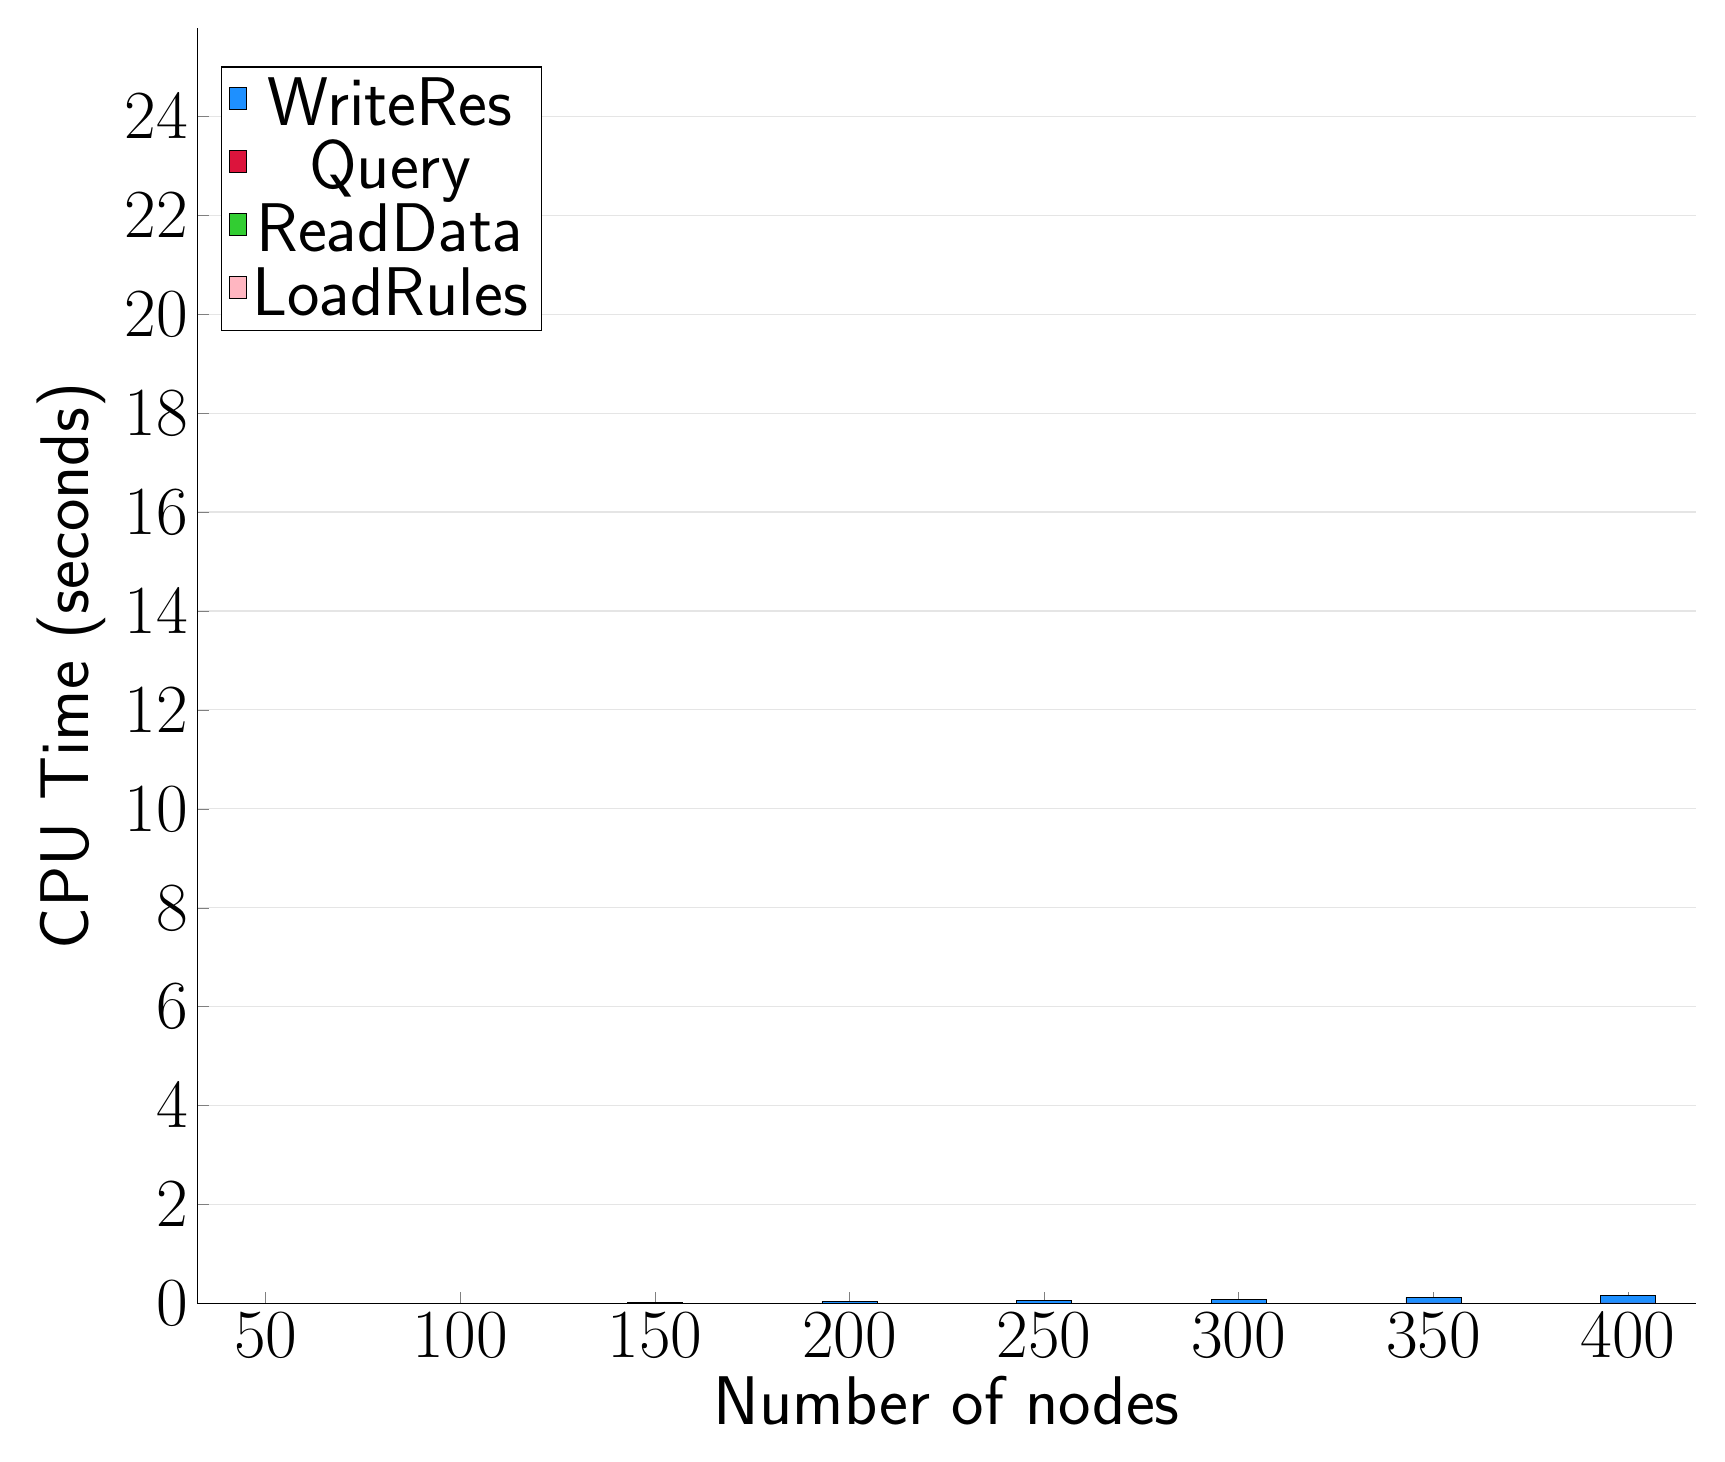
\begin{tikzpicture}
\begin{axis}[
   ybar stacked,
   width=1.7\textwidth,
   bar width=0.7cm,
   ymajorgrids, tick align=inside,
   major grid style={draw=gray!20},
   xtick=data,
   ymin=0, ymax=25.779619999999998,
   axis x line*=bottom,
   axis y line*=left,
   enlarge x limits=0.05,
   legend style={
       at={(0.23, 0.97)},
       anchor=north east,
       legend columns=1,
       font=\Huge,
   },
   ylabel={CPU Time (seconds)},
   xlabel={Number of nodes},
   label style={font=\Huge},
   tick label style={font=\Huge},
]
\addlegendimage{fill=DodgerBlue, draw=black, line width=0.2pt}
\addlegendentry{WriteRes}
\addlegendimage{fill=Crimson, draw=black, line width=0.2pt}
\addlegendentry{Query}
\addlegendimage{fill=LimeGreen, draw=black, line width=0.2pt}
\addlegendentry{ReadData}
\addlegendimage{fill=LightPink, draw=black, line width=0.2pt}
\addlegendentry{LoadRules}
\addplot +[fill=LightPink, draw=black, line width=0.2pt] coordinates {
(50, 0.0006333)
(100, 0.0005995)
(150, 0.0006054)
(200, 0.0006274999999999999)
(250, 0.0006001000000000001)
(300, 0.0006181999999999998)
(350, 0.0006144999999999998)
(400, 0.0006131000000000004)
};
\addplot +[fill=LimeGreen, draw=black, line width=0.2pt] coordinates {
(50, 0.0001802999999999996)
(100, 0.0002196999999999999)
(150, 0.00026230000000000014)
(200, 0.0003135999999999998)
(250, 0.00035130000000000024)
(300, 0.00039990000000000007)
(350, 0.00044700000000000046)
(400, 0.0004748999999999993)
};
\addplot +[fill=Crimson, draw=black, line width=0.2pt] coordinates {
(50, 0.0002576999999999999)
(100, 0.0009696999999999998)
(150, 0.0021565)
(200, 0.0038309999999999998)
(250, 0.005784600000000001)
(300, 0.0087443)
(350, 0.0119166)
(400, 0.015354399999999999)
};
\addplot +[fill=DodgerBlue, draw=black, line width=0.2pt] coordinates {
(50, 0.0023225000000000003)
(100, 0.009300600000000001)
(150, 0.0209035)
(200, 0.036817)
(250, 0.0573877)
(300, 0.08264429999999999)
(350, 0.1128278)
(400, 0.1456286)
};
\end{axis}
\end{tikzpicture}

\end{document}
